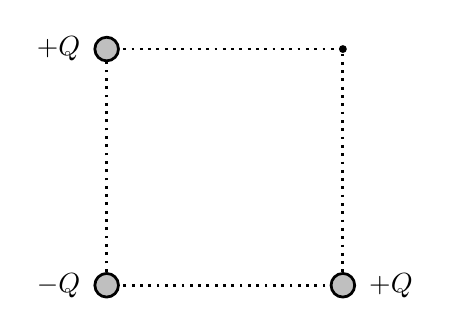
\begin{tikzpicture}[line width=1pt]
  \draw[dotted] (0,3) -- (3,3) -- (3,0) -- (0,0) -- cycle;
  \fill[gray!50] (0,3) circle (0.15);
  \draw (0,3) circle (0.15);
  \node[left] at (-0.2,3) {$+Q$};
  \fill (3,3) circle (0.05);
  \fill[gray!50] (0,0) circle (0.15);
  \draw (0,0) circle (0.15);
  \node[left] at (-0.2,0) {$-Q$};
  \fill[gray!50] (3,0) circle (0.15);
  \draw (3,0) circle (0.15);
  \node[right] at (3.2,0) {$+Q$};
\end{tikzpicture}
